\documentclass[a4paper,twoside]{article}
\usepackage[T1]{fontenc}
\usepackage[bahasa]{babel}
\usepackage{graphicx}
\usepackage{graphics}
\usepackage{float}
\usepackage[cm]{fullpage}
\pagestyle{myheadings}
\usepackage{etoolbox}
\usepackage{setspace} 
\usepackage{lipsum} 
\usepackage{amsmath}
\setlength{\headsep}{30pt}
\graphicspath{{./Gambar/}}% folder tempat gambar 
\usepackage[inner=2cm,outer=2.5cm,top=2.5cm,bottom=2cm]{geometry} %margin
% \pagestyle{empty}

\makeatletter
\renewcommand{\@maketitle} {\begin{center} {\LARGE \textbf{ \textsc{\@title}} \par} \bigskip {\large \textbf{\textsc{\@author}} }\end{center} }
\renewcommand{\thispagestyle}[1]{}
\markright{\textbf{\textsc{Laporan Perkembangan Pengerjaan Skripsi\textemdash Sem. Genap 2019/2020}}}

\onehalfspacing
 
\begin{document}

\title{\@judultopik}
\author{\nama \textendash \@npm} 

%ISILAH DATA BERIKUT INI:
\newcommand{\nama}{Stephen Jordan}
\newcommand{\@npm}{2016730018}
\newcommand{\tanggal}{25/11/2019} %Tanggal pembuatan dokumen
\newcommand{\@judultopik}{Penerapan Algoritma Anonimisasi Data pada Lingkungan Big Data} % Judul/topik anda
\newcommand{\kodetopik}{MTA4801}
\newcommand{\jumpemb}{2} % Jumlah pembimbing, 1 atau 2
\newcommand{\pembA}{Mariskha Tri Adithia, P.D.Eng}
\newcommand{\pembB}{Dr. Veronica Sri Moertini}
\newcommand{\semesterPertama}{48 - Genap 19/20} % semester pertama kali topik diambil, angka 1 dimulai dari sem Ganjil 96/97


\maketitle

\pagenumbering{arabic}

\section{Data Skripsi} %TIDAK PERLU MENGUBAH BAGIAN INI !!!
Pengambilan pertama kali topik ini pada : Semester {\bf \semesterPertama} \\
Pembimbing utama/tunggal: {\bf \pembA}\\
Pembimbing pendamping: {\bf \pembB}\\
Kode Topik : {\bf \kodetopik}


\section{Detail Perkembangan Pengerjaan Skripsi}
Detail bagian pekerjaan skripsi sesuai dengan rencan kerja/laporan perkembangan terkahir :
	\begin{enumerate}
		\item \textbf{Melakukan studi literatur mengenai konsep privasi, jenis-jenis privasi, konsep PII, contoh informasi yang bersifat sensitif dan non-sensitif menurut standar PII}\\
		{\bf Status :} Ada sejak rencana kerja skripsi.\\
		{\bf Hasil :} Privasi adalah suatu keadaan dimana kehidupan pribadi seseorang atau sekelompok orang terbebas dari pengawasan atau gangguan orang lain. Personally Identifiable Information (PII) adalah standar yang digunakan untuk menentukan apakah informasi yang ada dapat mengidentifikasi entitas individu. Contoh informasi sensitif menurut PII adalah identitas diri, nomor identitas diri, aset informasi (IP Address dan MAC Address). Contoh informasi non-sensitif menurut PII adalah rekaman medis, riwayat pendidikan, riwayat pekerjaan, informasi finansial.

		\item \textbf{Melakukan studi literatur mengenai teknik-teknik dasar data mining}\\
		{\bf Status :} Ada sejak rencana kerja skripsi.\\
		{\bf Hasil :} Data mining adalah proses menemukan korelasi, pola, dan tren baru yang bermakna dengan menyaring sejumlah besar data menggunakan teknologi pengenalan pola. Tahapan dalam data mining terdiri dari: selection, data preprocessing, transformation, data mining, intepretation/evaluation. Jenis pemodelan teknik data mining: klasifikasi dan pengelompokan/clustering. Klasifikasi adalah proses menemukan kelompok yang tepat dengan diberikan label kelas. Implementasi klasifikasi menggunakan pemodelan Naive Bayes. Pengelompokan/clustering adalah proses menganalisis kelompok data tanpa perlu mengetahui label kelas.  Implementasi clustering menggunakan pemodelan K-Means. Pada dokumen skripsi, telah dijelaskan kelebihan dan kekurangan setiap model data mining beserta langkah-langkah implementasinya secara singkat.
		
		\item \textbf{Melakukan studi literatur mengenai bidang studi lain terkait proses data mining beserta contoh penerapannya}\\
		{\bf Status :} Ada sejak rencana kerja skripsi.\\
		{\bf Hasil :} Jenis bidang studi terkait data mining yaitu visualisasi data, machine learning, dan statistika. Visualisasi adalah representasi data dalam bentuk grafik, umumnya data telah diringkas sebelum ditampilkan melalui grafik. Contoh dari bidang studi visualisasi data adalah line chart, bar chart, scatter plot, pie chart. Statistika adalah suatu metode yang digunakan dalam pengumpulan dan analisis data agar diperoleh informasi yang bermanfaat. Contoh dari bidang studi statistika adalah mean, median, modus, nilai maksimum dan minimum. Machine learning adalah metode pembelajaran pada sebuah komputer, agar komputer dapat belajar secara mandiri dan meningkatkan kinerjanya berdasarkan data pelatihan yang pernah diberi. Machine learning terdiri dari supervised learning dan unsupervised learning. Contoh penerapan supervised learning adalah klasifikasi. Contoh penerapan unsupervised learning adalah pengelompokan/clustering.
		
		\item \textbf{Melakukan studi literatur mengenai konsep Privacy Preserving Data Mining (PPDM), jenis perlindungan data, jenis serangan pada publikasi data}\\
		{\bf Status :} Ada sejak rencana kerja skripsi.\\
		{\bf Hasil :} Privacy Preserving Data Mining (PPDM) adalah teknik yang telah dikembangkan untuk mencegah pengungkapan informasi sensitif seseorang saat dilakukan data mining. Metode PPDM menjamin perlindungan data pada tingkat privasi tertentu bersamaan dengan memaksimalkan utilitas data, sehingga memungkinkan pengolahan data mining menghasilkan informasi yang efektif. Perlindungan data terjadi sebelum dilakukan pengumpulan data, proses data mining, publikasi data, distribusi data. Anonimisasi termasuk jenis perlindungan data untuk publikasi data. Implementasi anonimisasi berfokus pada pemodelan k-anonymity. Jenis serangan pada publikasi data terdiri dari record linkage, attribut linkage. Record linkage mengacu pada pemetaan beberapa data korban yang ditargetkan melalui hubungan antar data dalam sebuah tabel yang dirilis secara publik. Atribut linkage mengacu pada pemetaan beberapa data korban yang ditargetkan melalui hubungan antar atribut dalam sebuah tabel yang dirilis secara publik.
		
		\item \textbf{Melakukan studi literatur mengenai konsep anonimisasi dan jenis-jenis implementasi pada anonimisasi}\\
		{\bf Status :} Ada sejak rencana kerja skripsi.\\
		{\bf Hasil :} Anonimisasi adalah proses menghilangkan nilai atribut yang mengidentifikasi pribadi individu, baik secara langsung maupun tidak
langsung. Istilah umum yang digunakan dalam anonimisasi adalah Identifier (ID), Quasi-Identifier (QID), Equivalence class (EQ), Sensitive Attribute (SA), Non-sensitive Attribute (NSA). Berikut adalah jenis implementasi anonimisasi yang umum digunakan: anonimisasi berdasarkan generalisasi dan supresi, anonimisasi berdasarkan generalisasi, anonimisasi berdasarkan clustering. Pada dokumen skripsi, telah dipilih jenis implementasi anonimisasi berdasarkan clustering menggunakan pemodelan k-anonymity.

		\item \textbf{Melakukan studi literatur mengenai konsep k-anonymity dan jenis-jenis pendekatan algoritma pada K-Anonymity}\\
		{\bf Status :} Ada sejak rencana kerja skripsi.\\
		{\bf Hasil :} K-anonymity adalah pemodelan untuk mengurangi perbedaan antara satu data dengan data lain, agar sebuah data tidak dapat dibedakan setidaknya dengan k-1 data lainnya. K-anonymity memiliki tiga pendekatan yaitu algoritma k-means, algoritma k-member, dan algoritma greedy k-member clustering. Kekurangan dari algoritma k-means adalah pemilihan centroid awal  secara acak, sehingga setelah dilakukan generalisasi, hasil pengelompokannya mengakibatkan hilangnya informasi yang besar.  Kekurangan dari algoritma k-member adalah hanya mempertimbangkan pengelompokan terakhir tanpa memperhatikan pengelompokan yang dihasilkan pada proses sebelumnya sehingga menyebabkan distribusi kelompok pada beberapa bagian menjadi kurang tepat. Solusinya adalah menggabungkan kedua konsep dari algoritma k-means dan k-member menjadi sebuah algoritma baru yaitu greedy k-member clustering. Dengan menggunakan algoritma greedy k-member clustering, maka pengelompokan data dapat dilakukan satu kali sehingga dapat menurunkan kompleksitas algoritma dan hasil pemilihan centroid dapat dioptimalkan sehingga hasil pengelompokan dapat ditingkatkan secara signifikan.

\newpage
		\item \textbf{Melakukan studi literatur mengenai konsep, teorema, dan tahapan pada algoritma Greedy K-Member Clustering}\\
		{\bf Status :} Ada sejak rencana kerja skripsi.\\
		{\bf Hasil :} Algoritma greedy k-member clustering bertujuan untuk membagi seluruh data ke masing-masing kelompok data dengan kompleksitas dan utilitas data yang lebih baik dibandingkan algoritma clustering lain. Algoritma greedy k-member clustering memiliki tiga teorema yaitu: memiliki kompleksitas polinomial untuk kasus tertentu, setiap kelompok memiliki jumlah data sebanyak k buah data, jika jumlah data lebih besar daripada nilai k maka kompleksitasnya akan naik menjadi $O(n^2)$. Berikut adalah tahapan algoritma greedy k-member clustering pada dokumen skripsi:
		
\begin{figure}[H]
	\centering
	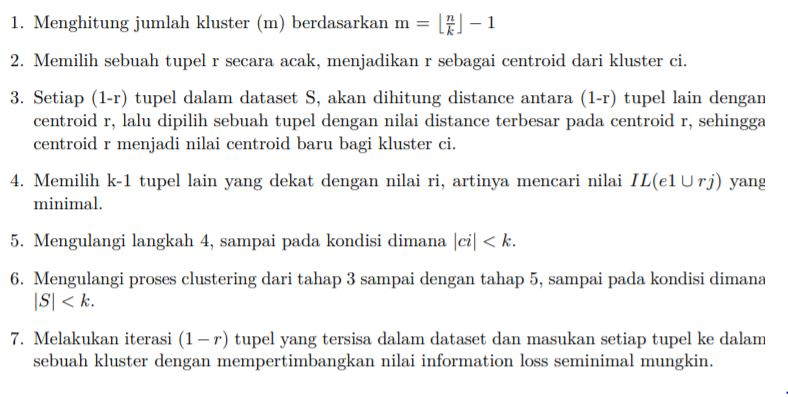
\includegraphics[scale=0.8]{algoritma}
	\caption{Tahapan Algoritma Greedy K-Member Clustering}
	\label{fig:algoritma}
\end{figure}

\item \textbf{Melakukan studi literatur mengenai metrik distance, information loss, dan cost function untuk pengujian anonimisasi}\\
		{\bf Status :} Ada sejak rencana kerja skripsi.\\
		{\bf Hasil :}  Anonimisasi diuji oleh tiga jenis metrik yaitu distance, information loss, dan cost function. Metrik dipakai
untuk mengukur kualitas data dan kinerja algoritma. Distance adalah  perhitungan untuk menyatakan akurasi data anonimisasi terhadap nilai data asli. Distance dipakai untuk mengukur tingkat perbedaan untuk masing-masing data dalam kelompok data yang sama. Perhitungan distance terdiri atas dua jenis yaitu: data numerik dan data kategorikal. Information Loss (IL) digunakan untuk mengevaluasi seberapa baik kinerja algoritma k- anonimisasi
terhadap nilai informasi sebuah data (utilitas data). Cost function berkaitan tentang efisiensi dan skalabilitas dari algoritma yang diterapkan untuk anonimisasi.

\item \textbf{Melakukan studi literatur mengenai konsep, manfaat, dan tantangan pada Sistem Terdistribusi}\\
		{\bf Status :} Ada sejak rencana kerja skripsi.\\
		{\bf Hasil :}  Sistem terdistribusi adalah kumpulan komputer berjalan secara independen, yang saling terhubung dan saling bekerja sama untuk mencapai satu tujuan yang sama. Manfaat sistem terdistribusi yaitu: horizontal scalability (pemrosesan komputasi skala besar), reliability (bergantung pada banyaknya komputer yang saling berkomunikasi satu sama lain), performance (komputasi pekerjaan lebih efisien karena beban kerja terbagi). Tantangan sistem terdistribusi yaitu: penjadwalan, latensi (waktu pertukaran data), observasi (kemampuan pengamatan kesalahan).

\newpage
\item \textbf{Melakukan studi literatur mengenai konsep dan jenis analisis pada Big Data}\\
		{\bf Status :} Ada sejak rencana kerja skripsi.\\
		{\bf Hasil :} Big data adalah data yang besar dan kompleks sehingga tidak mungkin sistem tradisional dapat memproses dan bekerja pada lingkungan data yang besar secara maksimal. Big data memiliki sifat 5V yaitu: volume, velocity, variety, veracity, value. Big data dapat dianalisis berdasarkan batch processing dan streaming processing. Batch processing adalah sekumpulan data disimpan terlebih dahulu, lalu pada waktu tertentu data yang telah terkumpul akan dilakukan analisis. Streaming processing adalah diasumsikan bahwa nilai informasi data yang diperoleh bergantung kepada seberapa cepat data dapat diolah secara real time.
		
		\item \textbf{Melakukan studi literatur mengenai konsep, ekosistem, arsitektur, dan komponen Hadoop}\\
		{\bf Status :} Ada sejak rencana kerja skripsi.\\
		{\bf Hasil :} Hadoop adalah framework yang melakukan pemrosesan data dengan memanfaatkan sistem terdistribusi dari kumpulan data besar yang terbagi pada seluruh komputer. Untuk melakukan analisis big data, Hadoop tidak bekerja sendiri. Ekosistem Hadoop bekerja sama dengan teknologi big data lain seperti Scoop, Flume, HBase, Pig, Hive, Mahout untuk melakukan analisis data tingkat lanjut seperti pemrosesan kueri SQL, machine learning, dan data collection. Arsitektur Hadoop terdiri dari master node dan slave node. Master node adalah node yang memberikan unit-unit pekerjaan kepada slave node. Slave node adalah node yang menuntaskan pekerjaan yang diberikan oleh master node. Hadoop memiliki empat element penting yaitu: NameNode, DataNode, JobTracker, TaskTracker. Keempat elemen penting ini tersebar pada seluruh komponen Hadoop. Hadoop memiliki dua komponen penting yaitu: HDFS, MapReduce. HDFS adalah sistem file terdistribusi pada Hadoop dengan menyediakan penyimpanan data yang handal, mendukung partisi, dan toleran terhadap kesalahan pemrosesan data pada hardware. Elemen penting pada HDFS yaitu NameNode dan DataNode. MapReduce adalah kerangka kerja pemrograman untuk komputasi terdistribusi yang dibuat oleh Google dengan membagi dan memecah masalah pekerjaan pada big data menjadi unit-unit kecil pekerjaan dan pemrosesan data secara paralel. Pada dokumen skripsi telah dijelaskan mengenai fungsi Mapper dan Reducer pada MapReduce. Elemen penting pada MapReduce yaitu JobTracker dan TaskTracker.
		
		\item \textbf{Melakukan studi literatur mengenai konsep, ekosistem,  arsitektur, jenis instalasi, operasi, dan komponen Spark}\\
		{\bf Status :} Ada sejak rencana kerja skripsi.\\
		{\bf Hasil :} Spark adalah alternatif dari Hadoop MapReduce untuk mengatasi keterbatasan pemrosesan input-output yang tidak efisien pada disk, dengan menggunakan memori. Untuk melakukan analisis big data, Spark tidak bekerja sendiri. Ekosistem Spark bekerja sama dengan library Spark dan teknologi big data lain seperti Cassandra, Kafka, ElasticSearch. Berikut adalah library Spark yang umum digunakan yaitu Spark SQL, Spark streaming, Spark MLlib, dan "GraphX". Library Spark dapat berjalan pada bahasa pemrograman tertentu seperti Java, Scala, dan Python. Arsitektur Spark terdiri dari driver program, cluster manager, dan worker. Driver Program adalah komputer yang sedang menjalankan perintah-perintah pada Spark. Cluster Manager  bertugas untuk mengatur jumlah pekerjaan yang diberikan untuk masing worker dan mengatur jumlah worker yang diperlukan. Spark memiliki tiga jenis instalasi yaitu standalone, Hadoop yarn, dan Spark In MapReduce(SIMR). Dari ketiga jenis instalasi tersebut, dipilih instalasi berdasarkan standalone karena paling simpel. Seluruh pekerjaan pada Spark dinyatakan dengan membuat RDD baru, mengubah RDD yang ada, atau memanggil operasi pada RDD untuk menghitung hasilnya. RDD adalah kumpulan data yang didistribusikan pada sistem terdistribusi. Jenis operasi pada RDD yaitu action dan tranformation. Komponen Spark adalah library tambahan pada Spark untuk melakukan proses komputasi pada
lingkungan big data berdasarkan jenis-jenis kebutuhan pengolahan data. Beberapa komponen Spark yang akan digunakan pada pengerjaan skripsi adalah Spark Core, Spark SQL, dan Spark MLlib. Spark Core adalah library dasar Spark yang harus disertakan untuk manipulasi objek RDD. Spark SQL adalah library  Spark untuk melakukan statistika pada data terstruktur seperti mean, median, modus. Spark MLlib adalah library Spark untuk melakukan proses data mining pada big data. 

\item \textbf{Melakukan studi literatur mengenai konsep, implementasi kode, dan GUI pada Scala}\\
		{\bf Status :} Ada sejak rencana kerja skripsi.\\
		{\bf Hasil :} Scala adalah bahasa pemrograman multi-paradigma yang mendukung paradigma pemrograman fungsional dan berorientasi objek pada lingkungan big data. Untuk pengembangan Spark, penulisan sintaks Scala dianggap produktif untuk mengimplementasikan kode program. Jenis variabel yang tersedia pada Scala adalah val dan var. Val adalah variabel yang tidak dapat diubah (seperti tipe "final" di Java). Var adalah variabel yang dapat diubah berdasarkan kebutuhan. Scala memiliki tipe data yang sama dengan bahasa pemrograman lain yaitu: boolean, byte, short, int, long, float, double, char. Struktur data pada Scala sering disebut sebagai collections. Struktur data Scala yang sering dipakai pada analisis big data adalah map dan list. Pada skripsi ini telah dicantumkan beberapa perintah scala yang umum digukanan sebagai berikut: implementasi object, kelas, main method, if-else, dan looping. Untuk GUI, Scala menyediakan library tambahan bernama Scala Swing. Scala Swing menyediakan komponen untuk merancang aplikasi seperti Frame, Panel, Label dan Button pada komponen GUI pada umumnya. Beberapa komponen pada Scala Swing dapat menangani handling event tertentu. Handling event adalah perkerjaan yang dilakukan sebuah komponen, ketika komponen tersebut menerima aksi dari pengguna.

		\item \textbf{Menulis dokumen skripsi}\\
		{\bf Status :} Ada sejak rencana kerja skripsi.\\
		{\bf Hasil :} Melakukan penulisan skripsi untuk bab 1 (pendahuluan) dan bab 2 (landasan teori). Pendahuluan berisi latar belakang masalah, rumusan masalah, tujuan penelitian, batasan masalah, metodologi, dan sistematika penulisan. Landasan teori berisi konsep, implementasi algoritma, langkah kerja, dan contoh implementasi terkait anonimisasi pada lingkungan big data.

	\end{enumerate}

\section{Pencapaian Rencana Kerja}
Langkah-langkah kerja yang berhasil diselesaikan dalam Skripsi 1 ini adalah sebagai berikut:
\begin{enumerate}
\item Mempelajari teknik-teknik dasar data mining
\item Mempelajari algoritma Greedy K-member clustering.
\item Mempelajari konsep Hadoop, Spark, dan Spark MLlib.
\item Menulis dokumen skripsi.
\end{enumerate}

\section{Kendala yang Dihadapi}
%TULISKAN BAGIAN INI JIKA DOKUMEN ANDA TIPE A ATAU C
Kendala - kendala yang dihadapi selama mengerjakan skripsi :
\begin{itemize}
	\item Library Spark untuk menangani jenis data XML tidak terlalu populer dan kurang dapat diandalkan.
	\item Beberapa istilah tidak tercantum dalam buku, sehingga menggunakan konsep dari jurnal orang lain.
	\item Terlalu banyak menghabiskan waktu untuk mencari buku dan jurnal terkait topik skripsi.
	\item Beberapa konsep belum pernah dipelajari pada matakuliah yang sudah/sedang diambil.
	\item Skripsi diambil bersamaan dengan matakuliah lain, dengan pengumpulan tugas besar.
	\item Pandemi COVID-19 di Indonesia mengganggu fokus pengerjaan skripsi.
\end{itemize}
	
\end{document}

